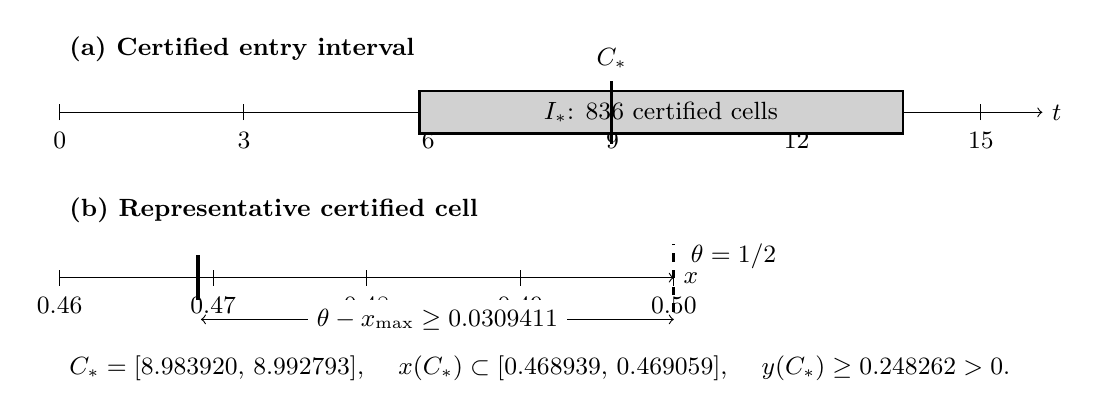
\begin{tikzpicture}[x=0.78cm,y=1cm,every node/.style={font=\small}]
  % Panel (a): full certified time interval
  \node[anchor=west,font=\small\bfseries] at (0,4.25)
    {(a) Certified entry interval};
  \draw[->] (0,3.45) -- (16,3.45) node[anchor=west] {\(t\)};
  \foreach \x/\lab in {0/0,3/3,6/6,9/9,12/12,15/15}{
    \draw (\x,3.35)--(\x,3.55);
    \node[below] at (\x,3.32) {\lab};
  }
  \fill[black!18] (5.857677,3.18) rectangle (13.727539,3.72);
  \draw[thick] (5.857677,3.18) rectangle (13.727539,3.72);
  \node at (9.79,3.45) {\(I_*\): 836 certified cells};

  % Representative cell, shown only as a marker
  \draw[very thick] (8.98835,3.05) -- (8.98835,3.85);
  \node[anchor=south] at (8.98835,3.88) {\(C_*\)};

  % Panel (b): prey enclosure against threshold
  \node[anchor=west,font=\small\bfseries] at (0,2.20)
    {(b) Representative certified cell};
  \draw[->] (0,1.35) -- (10.0,1.35) node[anchor=west] {\(x\)};
  \foreach \x/\lab in {0/0.46,2.5/0.47,5/0.48,7.5/0.49,10/0.50}{
    \draw (\x,1.25)--(\x,1.45);
    \node[below] at (\x,1.22) {\lab};
  }

  % x enclosure: map [0.46,0.50] to [0,10]
  \fill[black!35] (2.23470,1.08) rectangle (2.26472,1.62);
  \draw[thick] (2.23470,1.08) rectangle (2.26472,1.62);
  \draw[very thick,dashed] (10,0.92) -- (10,1.78);
  \node[anchor=west] at (10.12,1.62) {\(\theta=1/2\)};

  \draw[<->] (2.30,0.82) -- (10.0,0.82);
  \node[fill=white] at (6.15,0.82)
    {\(\theta-x_{\max}\ge 0.0309411\)};

  \node[anchor=west] at (0,0.20)
    {\(C_*=[8.983920,\,8.992793]\), \quad
      \(x(C_*)\subset[0.468939,\,0.469059]\), \quad
      \(y(C_*)\ge0.248262>0\).};
\end{tikzpicture}
